\documentclass{sigchi}

% Use this command to override the default ACM copyright statement
% (e.g. for preprints).  Consult the conference website for the
% camera-ready copyright statement.

%% HOW TO OVERRIDE THE DEFAULT COPYRIGHT STRIP --
%% Please note you need to make sure the copy for your specific
%% license is used here!
% \toappear{
% Permission to make digital or hard copies of all or part of this work
% for personal or classroom use is granted without fee provided that
% copies are not made or distributed for profit or commercial advantage
% and that copies bear this notice and the full citation on the first
% page. Copyrights for components of this work owned by others than ACM
% must be honored. Abstracting with credit is permitted. To copy
% otherwise, or republish, to post on servers or to redistribute to
% lists, requires prior specific permission and/or a fee. Request
% permissions from \href{mailto:Permissions@acm.org}{Permissions@acm.org}. \\
% \emph{CHI '16},  May 07--12, 2016, San Jose, CA, USA \\
% ACM xxx-x-xxxx-xxxx-x/xx/xx\ldots \$15.00 \\
% DOI: \url{http://dx.doi.org/xx.xxxx/xxxxxxx.xxxxxxx}
% }

% Arabic page numbers for submission.  Remove this line to eliminate
% page numbers for the camera ready copy
% \pagenumbering{arabic}

% Load basic packages
\usepackage{balance}       % to better equalize the last page
\usepackage{graphics}      % for EPS, load graphicx instead 
\usepackage[T1]{fontenc}   % for umlauts and other diaeresis
\usepackage{txfonts}
\usepackage{mathptmx}
\usepackage[pdflang={en-US},pdftex]{hyperref}
\usepackage{color}
\usepackage{booktabs}
\usepackage{textcomp}

\usepackage{dblfloatfix}

\usepackage{graphicx}
\usepackage{caption}
\usepackage{subcaption}
\usepackage{float}

% Some optional stuff you might like/need.
\usepackage{microtype}        % Improved Tracking and Kerning
% \usepackage[all]{hypcap}    % Fixes bug in hyperref caption linking
\usepackage{ccicons}          % Cite your images correctly!
% \usepackage[utf8]{inputenc} % for a UTF8 editor only

% If you want to use todo notes, marginpars etc. during creation of
% your draft document, you have to enable the "chi_draft" option for
% the document class. To do this, change the very first line to:
% "\documentclass[chi_draft]{sigchi}". You can then place todo notes
% by using the "\todo{...}"  command. Make sure to disable the draft
% option again before submitting your final document.
\usepackage{todonotes}

% Paper metadata (use plain text, for PDF inclusion and later
% re-using, if desired).  Use \emtpyauthor when submitting for review
% so you remain anonymous.
\def\plaintitle{SIGCHI Conference Proceedings Format}
\def\plainauthor{First Author, Second Author, Third Author,
  Fourth Author, Fifth Author, Sixth Author}
\def\emptyauthor{}
\def\plainkeywords{Game Design; Cooperative Game; Puzzle Solving; Unequal Communication Capabilities}
\def\plaingeneralterms{Documentation, Standardization}

% llt: Define a global style for URLs, rather that the default one
\makeatletter
\def\url@leostyle{%
  \@ifundefined{selectfont}{
    \def\UrlFont{\sf}
  }{
    \def\UrlFont{\small\bf\ttfamily}
  }}
\makeatother
\urlstyle{leo}

% To make various LaTeX processors do the right thing with page size.
\def\pprw{8.5in}
\def\pprh{11in}
\special{papersize=\pprw,\pprh}
\setlength{\paperwidth}{\pprw}
\setlength{\paperheight}{\pprh}
\setlength{\pdfpagewidth}{\pprw}
\setlength{\pdfpageheight}{\pprh}

% Make sure hyperref comes last of your loaded packages, to give it a
% fighting chance of not being over-written, since its job is to
% redefine many LaTeX commands.
\definecolor{linkColor}{RGB}{6,125,233}
\hypersetup{%
  pdftitle={\plaintitle},
% Use \plainauthor for final version.
%  pdfauthor={\plainauthor},
  pdfauthor={\emptyauthor},
  pdfkeywords={\plainkeywords},
  pdfdisplaydoctitle=true, % For Accessibility
  bookmarksnumbered,
  pdfstartview={FitH},
  colorlinks,
  citecolor=black,
  filecolor=black,
  linkcolor=black,
  urlcolor=linkColor,
  breaklinks=true,
  hypertexnames=false
}

% create a shortcut to typeset table headings
% \newcommand\tabhead[1]{\small\textbf{#1}}

% End of preamble. Here it comes the document.
\begin{document}

\newcommand{\getGameName}{Human and Dog}
\title{\getGameName\ : An Experiment on Unequal Communication Mechanic}

\numberofauthors{3}
\author{%
  \alignauthor{Leave Authors Anonymous\\
    \affaddr{for Submission}\\
    \affaddr{City, Country}\\
    \email{e-mail address}}\\
  \alignauthor{Leave Authors Anonymous\\
    \affaddr{for Submission}\\
    \affaddr{City, Country}\\
    \email{e-mail address}}\\
  \alignauthor{Leave Authors Anonymous\\
    \affaddr{for Submission}\\
    \affaddr{City, Country}\\
    \email{e-mail address}}\\
}

\maketitle

\begin{abstract}
  Inequality of communication capabilities like proficiency in a certain language may cause an awkward experience in real life. However, in terms of gaming, unequal communication mechanic can make games more challenging and interesting. \textit{Charades}\cite{Charades}, where one player tries to express a word via body language while the others try to guess it, is a good example of such cases. Hence, different from most cooperative digital games, which equal communication mechanic have been widely used, we experiment with this unequal communication mechanic. We have designed \getGameName, in which 2 players, a human and a dog, communicate to solve a series of puzzles with unequal communication capabilities.
%   Game design was explored through the information type.
%   "information type" too abstract
  Ultimately, we conducted an experiment to evaluate our game. 
%   From the collected data, several interesting communication patterns were discovered and we addressed some game design issues for future reference.
From our observation, several interesting communication patterns were discovered and we addressed some game design issues for future reference.
\end{abstract}

\category{K.8.0.}{General: Games}{}{}

\keywords{\plainkeywords}

\section{Introduction}
Cooperative design has been an integral part of many games, and one of the core mechanics is communication. Games with equal communication patterns can be widely seen, most of which adopt voice or text chat.
Others employ body language like \textit{Mute Robot}\cite{MuteRobot} and \textit{Way}\cite{Way} or pre-defined symbols like \textit{Portal 2}\cite{Portal2}.
On the contrary, cases where unequal communications happen seldom appear in the scenes of digital game design, while such situation regularly occurs in reality when people trying to communicate with deaf or mute people but knowing little about sign language, or even trying to communicate with pets.
Inspired by these real-world situations, we designed \getGameName, featuring two protagonists: one being a human, and the other being a dog. 
Each of them has asymmetric advantages that can be utilized to solve certain tasks and communicates with each other through unequal communication capabilities.
From this communication mechanic we addressed several factors regarding game challenges and communication patterns.
This paper is structured as follows: we summarize the research topics on communication patterns, mechanics, and how challenges affect players.
Next, we introduce the game design, including the game mechanics, the game design patterns and the description of the four levels.
Finally, we describe the game experiment used to evaluate our game, present the results, and discuss the findings.

\section{Related Work}
%Challenge second version
A challenge is considered to be one of the key components of game-play and has been an important research topic.
Cox et al. studied how the level of physical and cognitive challenge can affect a player's experience of immersion and concluded that a cognitive challenge may have greater effect on immersion \cite{Chall1}.
Iacovides et al. investigated how players actually overcome challenges and identified some player strategies \cite{Chall2}.
Both Cox and Iacovides quoted the Flow theory \cite{PsyFlow}, which suggests that flow is achieved as a result of an appropriate balance between the perceived level of challenges and the person's skills.

%Pattern exploration
Prior works have explored and analyzed cooperative game design patterns. Hsi et al. explored cooperative patterns within board games and yielded some observations that game designers might consider useful for designing collaborative game \cite{CG1}, and it also presented an ontology with a view to analyzing game play \cite{CG3}. 
Bjork and Holopainen presented a large quantity of game design patterns \cite{CG2}, including cooperative and social interaction patterns.
Rocha et al. presented a framework of several cooperative game design patterns and analyzed the actual impact of using these game mechanics to design a cooperative video game \cite{CG4}, which is later extended by El-Nasr et al. who proposed Cooperative Performance Metrics (CPMs) to evaluate game experiences \cite{CPMs}.
Also, Toups et al. analyzed the communication mechanics of 40 cooperative games using grounded theory \cite{CG5}.
Many communication patterns have been addressed in these past works, the unequal communication mechanic still yields some new and interesting patterns.

\section{Game Design}
%introduce the communication mechanics

%To present the inequality in communicative capabilities, the two playable characters in our game have been designed as a human and a dog respectively, both of which are equipped with different advantages and disadvantages.

%Since challenge is the key element in our communication mechanic, we identified several player strategies and understood which part of game-play may be a breakdown to players. Some hints were provided in some levels to balance the challenge and skill of some players. 

%introduce four different puzzles and their initial purpose
%first puzzle: communication for information
%second puzzle: communication for discrete spacial description (UDLR)
%third puzzle: communication for continuous spacial description in a 3D space
%fourth puzzle: communication for information, with aid of external tools (poker and periodic table)
Our game is a cooperative puzzle-solving game developed with Unity3D \cite{Unity}. The game involves two players at two different locations connected via Internet.
To enhance the interaction of two players, we adopted two cooperative game design patterns, \textit{Complementarity} and \textit{Information Asymmetry}.
% \textit{Complementarity}, which was also identified in Rocha's et al work \cite{CG4}, implies that players play difference roles to complement each others' activities within the game. 
\textit{Complementarity}, defined by Rocha et al. \cite{CG4}, implies that players play different roles to complement each others' activities within the game. 
\textit{Information Asymmetry} indicates that different players would acquire and perceive different information during game-play.
Furthermore, the most important mechanic of our game is the unequal communication.
We experiment this mechanic with two player characters, a human and a dog character described below:

\begin{itemize}
\item \textbf{Human Character}\newline
The human is able to operate intricate moves such as tapping a keypad or typing a computer.
Also, the character can use verbal language to communicate with the other player.
\item \textbf{Dog Character}\newline
The dog has a different range of sensing capabilities regarding olfaction and vision, and thus certain clues can only be detected by this character.
Also, it is capable of passing through narrow areas due to its smaller figure.
In the setting of our game, the dog was transformed from a human.
Although it can understand what the human is saying, its communication capabilities are limited to 4 different kinds of vocal patterns (whine, howl, bark, and anger.)
\end{itemize}

\subsection{Level Design}

In terms of level design, our goal is to explore the game design with the information type and examine how players exchange different types of information. The description of these levels is outlined below:

\begin{enumerate}

\item \textbf{Symbolic information problem}\newline
% The first puzzle is inputting the correct code in a keypad on a wall.
The first puzzle is to guess the password of a door by pressing numbers of a keypad on a wall.
% The human needs to figure out the permutation of the digits according to the clue on nearby desk and the dog will find out the digits which constitute the code by sniffing the dead scientist and then the keypad.
The human needs to figure out the digit sequence according to the clue on a nearby desk, and the dog looks for the digits which constitute the code by sniffing the dead scientist and then the keypad. (\autoref{fig:keypad_and_name} {\textbf{(a)} and {\textbf{(b)})

\item \textbf{Discrete spatial information problem}\newline
% The second puzzle is a modified 8-puzzle \cite{8puzzle}, where the picture on it is unseen by the human, while the dog can find the clue and see the picture of the puzzle on the opposite side by passing through a narrow aisle. (\autoref{fig:8puzzle} and \autoref{fig:puzzle2_view})
There are two parts of the second puzzle.
The first part is to look for a narrow secret passage way that only fits the size of a dog.
After the dog passes through the passage, both the human and the dog must communicate from different rooms to solve the second part of the puzzle. (\autoref{fig:puzzle2_all} {\textbf{(c)})
The second part is a modified 8-puzzle where the side with no picture faces the human and the side with a picture faces the dog, and therefore the dog instructs the human to move the tiles.  (\autoref{fig:puzzle2_all} {\textbf{(a)} and {\textbf{(b)})
%May need to explain why the human knew the existence of the mushrooms.
\item \textbf{Continuous spatial information problem}\newline
% The third puzzle requires two players to destroy three mushrooms located in the room. These mushrooms are invisible to the human, but not the dog. However, the only way to destroy them is by shooting bullets at them, which can be done only by the human. 
The third puzzle is a first person shooting game for the human with the objective of mushroom destruction.
However, there are 3 genetically-modified mushrooms only visible to the dog but invisible to the human. (\autoref{fig:auxiliaryItems_and_mushrooms} {\textbf{(b)} and {\textbf{(c)})
The dog must show the locations of the mushrooms for the human to shoot at in order to complete the puzzle.

\item \textbf{Auxiliary items represented information problem}\newline
In the last puzzle, players are provided with auxiliary items: a set of poker cards and a periodic table.(\autoref{fig:auxiliaryItems_and_mushrooms} {\textbf{(a)}) A name written in English alphabets can only be discovered by the dog nearby a dead scientist (\autoref{fig:keypad_and_name} {\textbf{(c)}) and is the password for accessing a computer which can only be operated by the human. 
\end{enumerate}

% \begin{figure}[H]
%     \minipage[t]{0.5\linewidth}
%         \centering
%         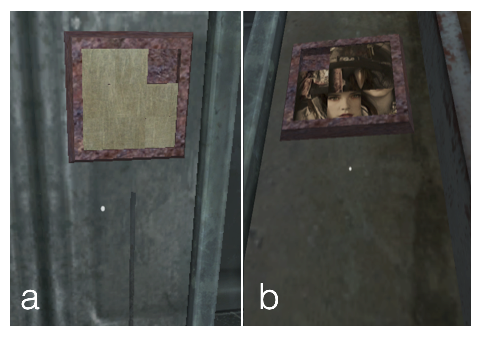
\includegraphics[width=\linewidth]{images/8puzzle.png}
%         \caption{The modified 8-puzzle:  \textbf{(a)} the human's view \textbf{(b)}  the dog's view}
%         \label{fig:8puzzle}
%     \endminipage
%     ~ %add desired spacing between images, e. g. ~, \quad, \qquad, \hfill etc. 
%       %(or a blank line to force the minipage onto a new line)
%     \minipage[t]{0.5\linewidth}
%         \centering
%         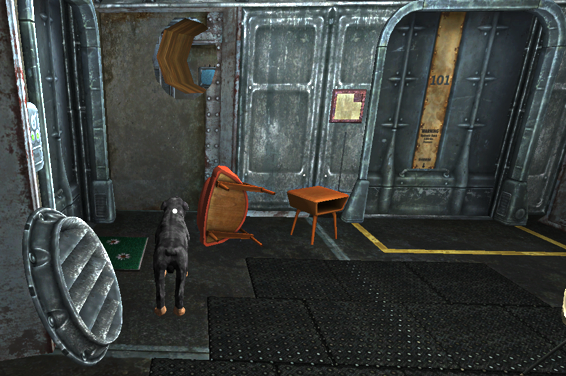
\includegraphics[width=\linewidth]{images/puzzle2_view.png}
%         \caption{the view of second puzzle and the narrow aisle}
%         \label{fig:puzzle2_view}
%     \endminipage
%     ~ %add desired spacing between images, e. g. ~, \quad, \qquad, \hfill etc. 
%     %(or a blank line to force the minipage onto a new line)
% \end{figure}

\begin{figure}[H]
\centering
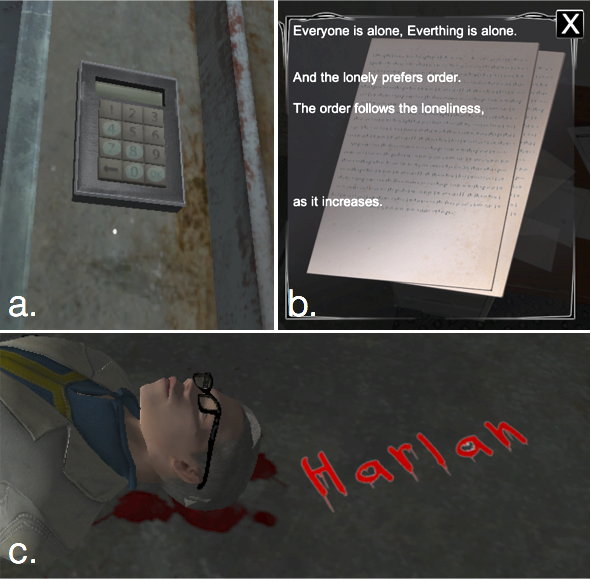
\includegraphics[width=0.7\linewidth]{images/puzzle1_and_4.png}
\caption{\textbf{(a)}: The keypad from dog's view. \textbf{(b)}: The clue on the nearby desk. \textbf{(c)}: The name that can only be seen by dog.}
\label{fig:keypad_and_name}
\end{figure}

\begin{figure}[H]
\centering
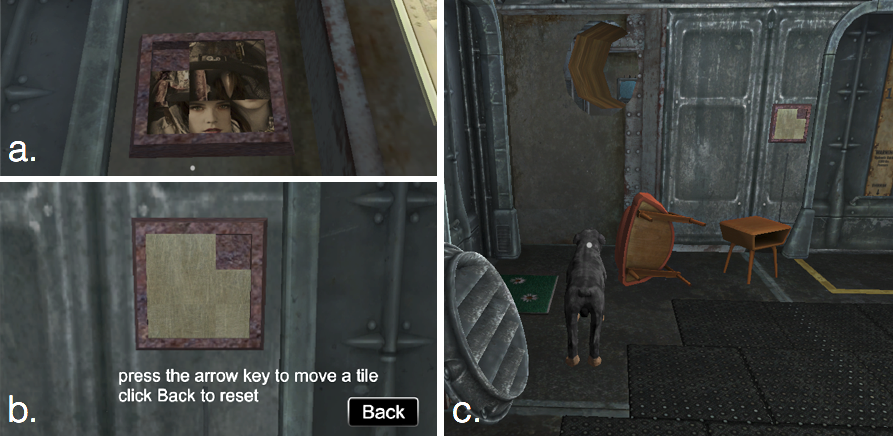
\includegraphics[width=0.9\linewidth]{images/puzzle2_all.png}
\caption{\textbf{(a)} \& \textbf{(b)}: The modified 8-puzzle seen on the side of human and dog, respectively. \textbf{(c)}: The passage that only the dog can pass through.}
\label{fig:puzzle2_all}
\end{figure}

\begin{figure}[H]
\centering
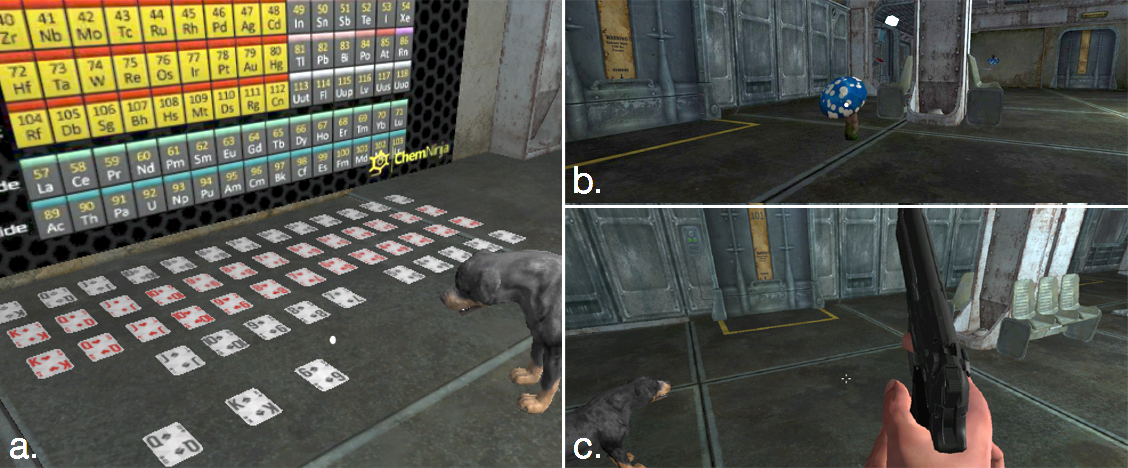
\includegraphics[width=0.9\linewidth]{images/puzzle3_and_4.png}
\caption{\textbf{(a)} The auxiliary items: poker cards and periodic table. \textbf{(b)} \& \textbf{(c)}: The mushroom in the dog's and the human's view respectively.}
\label{fig:auxiliaryItems_and_mushrooms}
\end{figure}

% \begin{figure}[H]
%     \minipage[t]{0.5\linewidth}
%         \centering
%         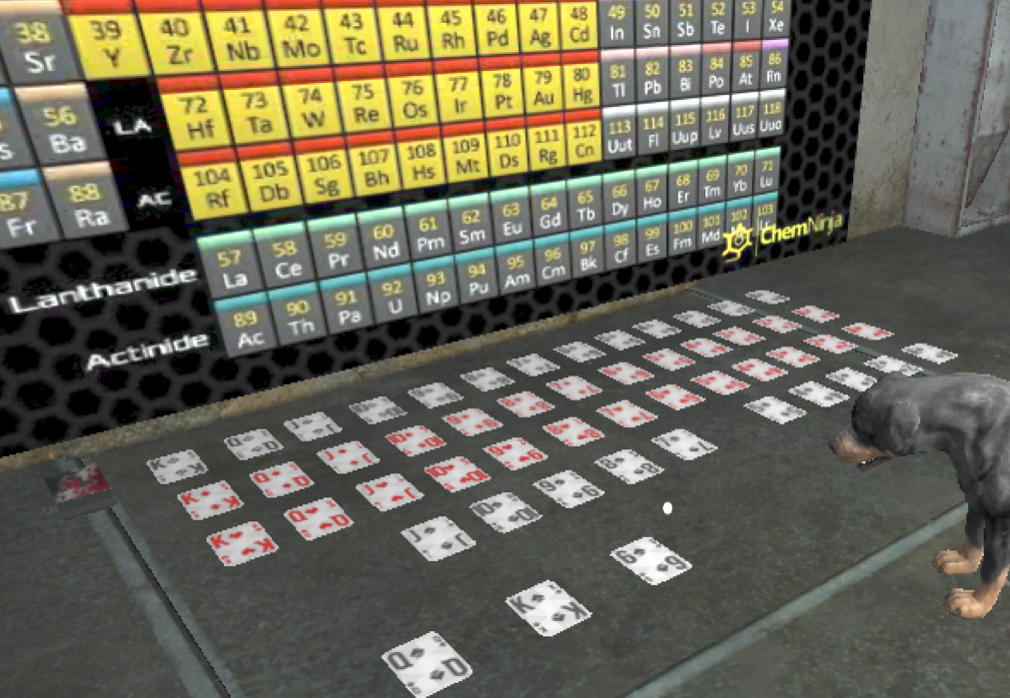
\includegraphics[width=\linewidth]{images/auxiliary_items.png}
%         \caption{The auxiliary items: poker cards and periodic table.}
%         \label{fig:auxiliary_items}
%     \endminipage
%     ~ %add desired spacing between images, e. g. ~, \quad, \qquad, \hfill etc. 
%       %(or a blank line to force the minipage onto a new line)
%     \minipage[t]{0.5\linewidth}
%         \centering
%         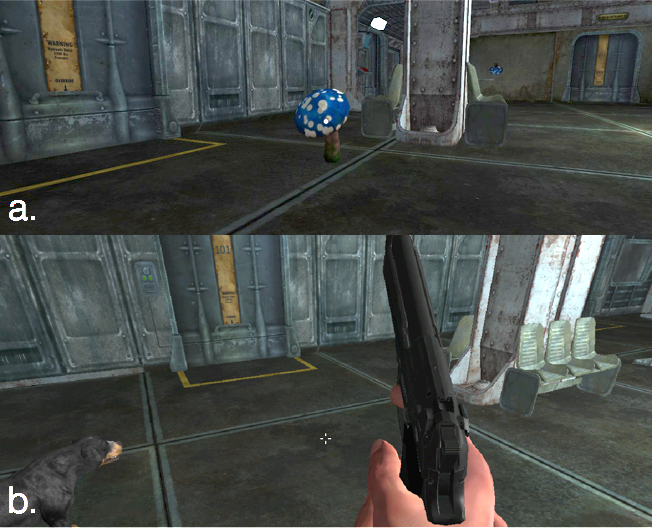
\includegraphics[width=\linewidth]{images/puzzle3_2.png}
%         \caption{The mushroom: \textbf{(a)}  the dog's view \textbf{(b)} the human's view}
%         \label{fig:puzzle3}
%     \endminipage
%     ~ %add desired spacing between images, e. g. ~, \quad, \qquad, \hfill etc. 
%     %(or a blank line to force the minipage onto a new line)
% \end{figure}

\section{Study Design}
% In order to understand the behaviours and experience of players, 16 participants were recruited (F=5;M=11;Age=20 to 27). Before they started playing, we told them the input and the rules of the game. The characters were randomly assigned and the duration of game-play was around 40 to 50 minutes. After they finished the game-play, we let them do a brief questionnaire about their gaming habits, a 5 points Likert-scale questionnaire to collect their experience, such as difficulty and enjoyment, during the game-play and did a short interviewed with them to understand their strategies, communication protocols and behaviours in some special situations.
In order to understand user behaviours and the gaming experience of our game design, 16 participants were recruited (F=5;M=11;Age=20 to 27).
Before they started, operations for both the human and dog player character and the rules of the game were introduced.
The human and dog characters were randomly assigned and the duration of game-play was around 40 to 50 minutes.
After the game-play, the participants filled up a brief questionnaire about their gaming habits and a 5-point Likert-scale questionnaire to collect their game-play experience of \getGameName{} such as difficulty and enjoyment. 
We also conducted a short interview with them to understand their strategies, communication protocols, and behaviours in some certain situations.
\section{Result}
We received overall positive feedbacks from the participants. The average enjoyment of each puzzles is all rated high (above 3.75 out of 5.0). As for the difficulty aspect, players as human find the last two levels more difficult specifically on communicating with the other player, but the second puzzle holds the most difficult one in terms of overall difficulty. Players as dogs, however, finds communicating most difficult in the second puzzle, and the overall difficulty result shows that the last puzzle are considered the most difficult.
\begin{figure}[h]
\centering
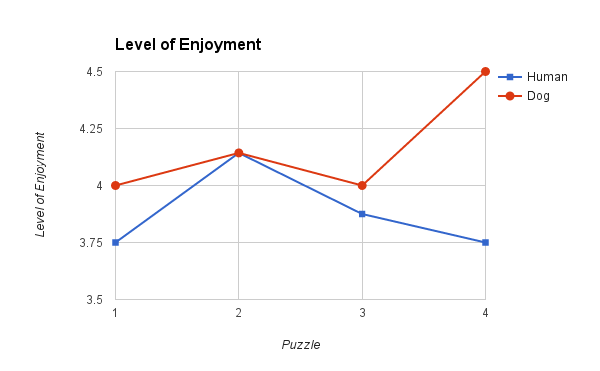
\includegraphics[width=0.9\linewidth]{images/enjoyment.png}
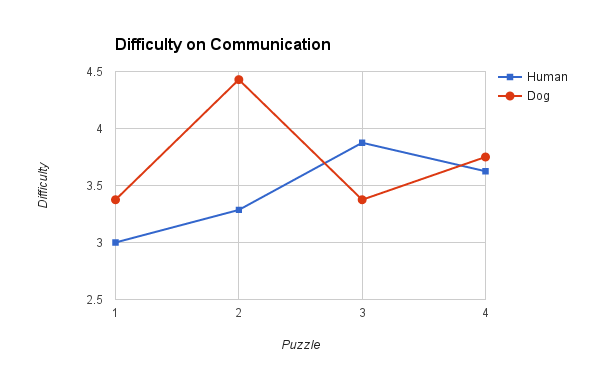
\includegraphics[width=0.9\linewidth]{images/communication_difficulty.png}
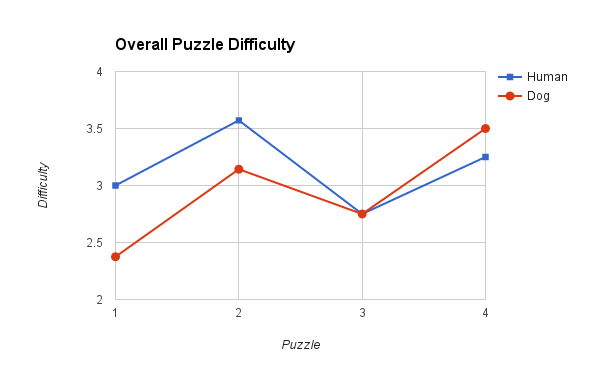
\includegraphics[width=0.9\linewidth]{images/overall_difficulty.png}
\end{figure}
\section{Discussion}
\subsection{Communication Patterns}
After observing the game-play of sixteen participants and interviewing with them, we identified various communication patterns and outlines them below:
\begin{enumerate}
\item \textbf{Mapping dog vocal patterns to certain meanings}\newline
% Usually at the beginning of the game, players would settle down the mapping of yes and no, either to the number of voice, such as "if it's yes then bark once; otherwise, bark twice.", or to the feeling of an voice by instinct, such as "if it's yes then bark; otherwise, whine or use the angry voice." In the first puzzle, some of the human players would map the digits in the way of "The occurrence of barking represent the next digit." or ask a yes-no question about whether the next digit is a certain number. In the second puzzle, most of the human players would mapping the next direction to the number of voice or the feeling of an voice. A few would map the position of a tile to the number of voice.
Usually at the beginning of the game, players would settle down the mapping of positive and negative.
Some distinguish positive and negative by the number of voice or by the 4 vocal patterns of the dog.
For example, ``If the answer is yes, then bark once; otherwise, bark twice.''
For another example, ``If it's yes, then bark; otherwise, whine or use the angry voice.''
In the first puzzle, some of the human players would map the digits by the number of occurrence of barking to represent a digit or ask a yes-no question about whether the next digit is a certain number.
In the second puzzle, most of the human players would map the next direction to the number of dog voice or the feeling of an voice.
A few would map the position of a tile to the number of voice.
In the third puzzle, the human players may iteratively correct their aiming direction by asking ``Should I aim upward,downward,leftward or rightward'' and shoot until they have shot a mushroom.

% \item \textbf{From macro to micro}\newline
\item \textbf{Narrowing Down}\newline
% third puzzle : on the wall or on the floor
% how many alphabets are in the name?
% Is the elements in the first group?
% We also observed that some of the human players would ask some questions to narrow the information space. For example, in third puzzle, the human players would ask "Is the mushroom on the ground or on the wall?". In the last puzzle, the human players would ask how many alphabets are in the name first and when they were communicating via periodic table, some of the human players would ask "Is the  indicated element in the first group?".
We also observed that some of the human players would ask some questions to narrow down possibilities.
For example, in the third puzzle, the human players would ask ``Is the mushroom on the ground or on the wall?''.
In the last puzzle, the human players would ask how many alphabets are in the name first and when they were communicating via periodic table, some of the human players would ask ``Is the indicated element in the first group?''.

\item \textbf{Taking turns in the leading position}\newline
% third puzzle : lead the way
% last puzzle : dog would actively pick the cards and human would guess the mapping rule defined by dog.
% drawing attention
% Most of the time, the human players would take the leading position. However, the dog may discover the key information to the puzzle first and it would try to draw the attention of the human with its sound. For instance, in the third puzzle, the human couldn't know the locations of the mushrooms so they would let the dog lead the way. In the last puzzle, some of the dog players would actively pick the poker cards and the human players would guess what kinds of rules the dog tried to convey.
Most of the time, the human players would take the leading position.
However, the dog may discover the key information to the puzzle first, and it would try to draw the attention of the human with its sound.
For instance, in the third puzzle, the human did not know the locations of the mushrooms so they would let the dog lead the way.
In the last puzzle, some of the dog players would actively pick the poker cards and the human players would guess what kinds of rules the dog managed to convey.

\item \textbf{Expressing through body language}\newline
Except the dog would express the information with its sound, it may also use certain kinds of body language. 
For example, in the third puzzle, the human players would guess the location of a mushroom based on the facing direction of the dog since this information was also synchronized in the system. Some of the dog players may use jumping to indicate there is something around its current location or something on the wall with higher position. For example, in the last puzzle, the dog player would use jumping to express that the element with smaller atomic number is in the group aligned with the dog's location.

\item \textbf{Communicating with auxiliary items}\newline
In the last puzzle, a set of poker cards and a periodic table were provided to help communication. Players would use poker cards to represent a certain number. Two kinds of behaviour were observed. One is the numeric value of a card corresponding to one of the digits of the number and one is the sum of the numeric values of cards representing the number. In addition, the number would be the order of an alphabet in the name or the atomic value of an element, which further represent an alphabet in the name. Other interesting mappings were also discovered like using one of suits of cards to represent the group number of elements and another one to represent the period of elements.

%body language
%auxiliary items
\end{enumerate}

\subsection{Design Issues}
After observing the game-play of sixteen participants and interviewing with them, we have discovered some game issues under the unequal communication mechanic.

\begin{enumerate}
\item \textbf{Narrowing the information gap}\newline
Although Information Asymmetry is pretty common in many cooperative games, there is a challenge in our communication mechanic. This challenge would require the human player iteratively ask questions to shape his own understanding of the key information the dog player has. If the human players is not good at this kind of communication or the key information is beyond his understanding, they would feel pretty frustrated. To address this issue, there are two approaches. First one is placing a hint to help the human player shape his own understanding. The other one is enhancing the communication capability of the dog player under the no-direct-voice constrain, such as visualizing where the dog is looking at while it is barking. 

\item \textbf{Avoiding making a puzzle too complex}\newline
In the second puzzle, some human players have pretty diverse imagination of what the dog see at the opposite side of the room. The information gap would be too large to them. Hence, a hint was provided to the human for addressing this issue.

\item \textbf{Avoiding repetitive tasks for players}\newline
After doing the quantitative analysis, we found that there is a positive correlation between the enjoyment of the dog and the overall difficulty of the dog in each puzzle. But there is a drop between the enjoyment of the human and the overall difficulty of the human in the last puzzle. A possible reason for this may be that repetitive tasks are needed to solve this puzzle (i.e. asking for the correct alphabet), which lowers down the enjoyment. This can also explain why the second puzzle has the highest enjoyment within the four, where the answer is the shortest (4 steps to solve the puzzle), and requires the least queries.

\end{enumerate}

\section{Conclusion}
In this paper, we present a game experimenting with the unequal communication mechanic, which few games have explored before. We explored the game design with the information type and conducted a game experiment to evaluate our game and understand players' behaviour and experience. Finally, we identified various communication patterns and addressed some game issues for future reference. We hope to see more future work experimenting with this mechanic.

\bibliographystyle{SIGCHI-Reference-Format}
\bibliography{sample}

\end{document}

%------------------
% original template
%------------------

% \section{Page Size and Columns}
% On each page your material should fit within a rectangle of 7 $\times$
% 9.15 inches (18 $\times$ 23.2 cm), centered on a US Letter page (8.5
% $\times$ 11 inches), beginning 0.85 inches (1.9 cm) from the top of
% the page, with a 0.3 inches (0.85 cm) space between two 3.35 inches
% (8.4 cm) columns. Right margins should be justified, not
% ragged. Please be sure your document and PDF are US letter and not A4.

% \section{Typeset Text}
% The styles contained in this document have been modified from the
% default styles to reflect ACM formatting conventions. For example,
% content paragraphs like this one are formatted using the Normal style.

% \LaTeX\ sometimes will create overfull lines that extend into columns.
% To attempt to combat this, the \texttt{.cls} file has a command,
% \texttt{{\textbackslash}sloppy}, that essentially asks \LaTeX\ to
% prefer underfull lines with extra whitespace.  For more details on
% this, and info on how to control it more finely, check out
% {\url{http://www.economics.utoronto.ca/osborne/latex/PMAKEUP.HTM}}.

% \subsection{Title and Authors}

% Your paper's title, authors and affiliations should run across the
% full width of the page in a single column 17.8 cm (7 in.) wide.  The
% title should be in Helvetica or Arial 18-point bold.  Authors' names
% should be in Times New Roman or Times Roman 12-point bold, and
% affiliations in 12-point regular.  

% See \texttt{{\textbackslash}author} section of this template for
% instructions on how to format the authors. For more than three
% authors, you may have to place some address information in a footnote,
% or in a named section at the end of your paper. Names may optionally
% be placed in a single centered row instead of at the top of each
% column. Leave one 10-point line of white space below the last line of
% affiliations.

% \subsection{Abstract and Keywords}

% Every submission should begin with an abstract of about 150 words,
% followed by a set of Author Keywords and ACM Classification
% Keywords. The abstract and keywords should be placed in the left
% column of the first page under the left half of the title. The
% abstract should be a concise statement of the problem, approach, and
% conclusions of the work described. It should clearly state the paper's
% contribution to the field of HCI\@.

% \subsection{Normal or Body Text}

% Please use a 10-point Times New Roman or Times Roman font or, if this
% is unavailable, another proportional font with serifs, as close as
% possible in appearance to Times Roman 10-point. Other than Helvetica
% or Arial headings, please use sans-serif or non-proportional fonts
% only for special purposes, such as source code text.

% \subsection{First Page Copyright Notice}
% This template include a sample ACM copyright notice at the bottom of
% page 1, column 1.  Upon acceptance, you will be provided with the
% appropriate copyright statement and unique DOI string for publication.
% Accepted papers will be distributed in the conference
% publications. They will also be placed in the ACM Digital Library,
% where they will remain accessible to thousands of researchers and
% practitioners worldwide. See
% \url{http://acm.org/publications/policies/copyright_policy} for the
% ACM's copyright and permissions policy.

% \subsection{Subsequent Pages}

% On pages beyond the first, start at the top of the page and continue
% in double-column format.  The two columns on the last page should be
% of equal length.



% \subsection{References and Citations}

% Use a numbered list of references at the end of the article, ordered
% alphabetically by last name of first author, and referenced by numbers
% in
% brackets~\cite{acm_categories,ethics,Klemmer:2002:WSC:503376.503378}.
% Your references should be published materials accessible to the
% public. Internal technical reports may be cited only if they are
% easily accessible (i.e., you provide the address for obtaining the
% report within your citation) and may be obtained by any reader for a
% nominal fee. Proprietary information may not be cited. Private
% communications should be acknowledged in the main text, not referenced
% (e.g., ``[Borriello, personal communication]'').

% References should be in ACM citation format:
% \url{http://acm.org/publications/submissions/latex_style}. This
% includes citations to internet
% resources~\cite{acm_categories,cavender:writing,CHINOSAUR:venue,psy:gangnam}
% according to ACM format, although it is often appropriate to include
% URLs directly in the text, as above.

% Use a numbered list of references at the end of the article, ordered
% alphabetically by first author, and referenced by numbers in
% brackets~\cite{ethics, Klemmer:2002:WSC:503376.503378,
%   Mather:2000:MUT, Zellweger:2001:FAO:504216.504224}. For papers from
% conference proceedings, include the title of the paper and an
% abbreviated name of the conference (e.g., for Interact 2003
% proceedings, use \textit{Proc. Interact 2003}). Do not include the
% location of the conference or the exact date; do include the page
% numbers if available. See the examples of citations at the end of this
% document. Within this template file, use the \texttt{References} style
% for the text of your citation.

% Your references should be published materials accessible to the
% public.  Internal technical reports may be cited only if they are
% easily accessible (i.e., you provide the address for obtaining the
% report within your citation) and may be obtained by any reader for a
% nominal fee.  Proprietary information may not be cited. Private
% communications should be acknowledged in the main text, not referenced
% (e.g., ``[Robertson, personal communication]'').

% \begin{table}
%   \centering
%   \begin{tabular}{l r r r}
%     % \toprule
%     & & \multicolumn{2}{c}{\small{\textbf{Test Conditions}}} \\
%     \cmidrule(r){3-4}
%     {\small\textit{Name}}
%     & {\small \textit{First}}
%       & {\small \textit{Second}}
%     & {\small \textit{Final}} \\
%     \midrule
%     Marsden & 223.0 & 44 & 432,321 \\
%     Nass & 22.2 & 16 & 234,333 \\
%     Borriello & 22.9 & 11 & 93,123 \\
%     Karat & 34.9 & 2200 & 103,322 \\
%     % \bottomrule
%   \end{tabular}
%   \caption{Table captions should be placed below the table. We
%     recommend table lines be 1 point, 25\% black. Minimize use of
%     table grid lines.}~\label{tab:table1}
% \end{table}

% \section{Sections}

% The heading of a section should be in Helvetica or Arial 9-point bold,
% all in capitals. Sections should \textit{not} be numbered.

% \subsection{Subsections}

% Headings of subsections should be in Helvetica or Arial 9-point bold
% with initial letters capitalized.  For sub-sections and
% sub-subsections, a word like \emph{the} or \emph{of} is not
% capitalized unless it is the first word of the heading.

% \subsubsection{Sub-subsections}

% Headings for sub-subsections should be in Helvetica or Arial 9-point
% italic with initial letters capitalized.  Standard
% \texttt{{\textbackslash}section}, \texttt{{\textbackslash}subsection},
% and \texttt{{\textbackslash}subsubsection} commands will work fine in
% this template.

% \section{Figures/Captions}

% Place figures and tables at the top or bottom of the appropriate
% column or columns, on the same page as the relevant text (see
% Figure~\ref{fig:figure1}). A figure or table may extend across both
% columns to a maximum width of 17.78 cm (7 in.).

% \begin{figure*}
%   \centering
%   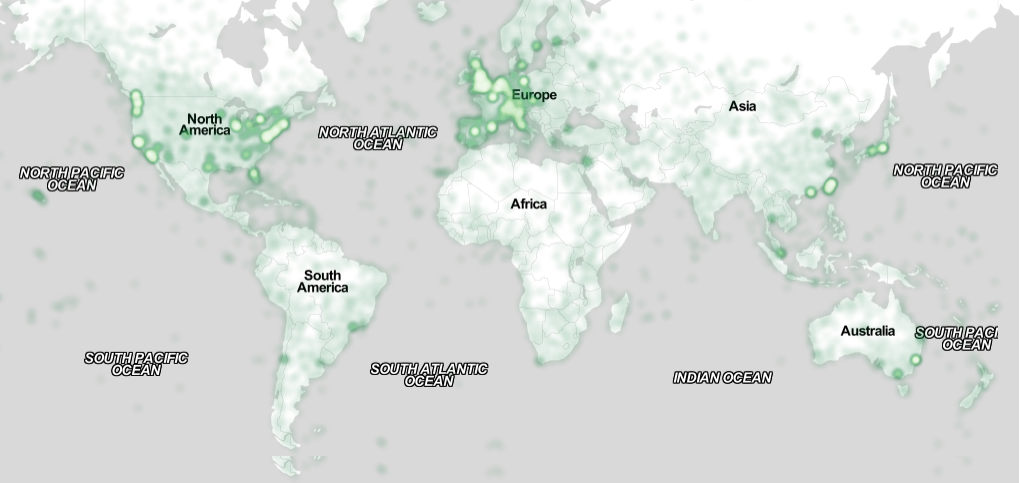
\includegraphics[width=1.75\columnwidth]{figures/map}
%   \caption{In this image, the map maximizes use of space. You can make
%     figures as wide as you need, up to a maximum of the full width of
%     both columns. Note that \LaTeX\ tends to render large figures on a
%     dedicated page. Image: \ccbynd~ayman on
%     Flickr.}~\label{fig:figure2}
% \end{figure*}

% Captions should be Times New Roman or Times Roman 9-point bold.  They
% should be numbered (e.g., ``Table~\ref{tab:table1}'' or
% ``Figure~\ref{fig:figure1}''), centered and placed beneath the figure
% or table.  Please note that the words ``Figure'' and ``Table'' should
% be spelled out (e.g., ``Figure'' rather than ``Fig.'') wherever they
% occur. Figures, like Figure~\ref{fig:figure2}, may span columns and
% all figures should also include alt text for improved accessibility.
% Papers and notes may use color figures, which are included in the page
% limit; the figures must be usable when printed in black-and-white in
% the proceedings.

% The paper may be accompanied by a short video figure up to five
% minutes in length. However, the paper should stand on its own without
% the video figure, as the video may not be available to everyone who
% reads the paper.  

% \subsection{Inserting Images}
% When possible, include a vector formatted graphic (i.e. PDF or EPS).
% When including bitmaps,  use an image editing tool to resize the image
% at the appropriate printing resolution (usually 300 dpi).

% \section{Quotations}
% Quotations may be italicized when \textit{``placed inline''} (Anab,
% 23F).

% \begin{quote}
% Longer quotes, when placed in their own paragraph, need not be
% italicized or in quotation marks when indented (Ramon, 39M).  
% \end{quote}

% \section{Language, Style, and Content}

% The written and spoken language of SIGCHI is English. Spelling and
% punctuation may use any dialect of English (e.g., British, Canadian,
% US, etc.) provided this is done consis- tently. Hyphenation is
% optional. To ensure suitability for an international audience, please
% pay attention to the following:

% \begin{itemize}
% \item Write in a straightforward style.
% \item Try to avoid long or complex sentence structures.
% \item Briefly define or explain all technical terms that may be
%   unfamiliar to readers.
% \item Explain all acronyms the first time they are used in your
%   text---e.g., ``Digital Signal Processing (DSP)''.
% \item Explain local references (e.g., not everyone knows all city
%   names in a particular country).
% \item Explain ``insider'' comments. Ensure that your whole audience
%   understands any reference whose meaning you do not describe (e.g.,
%   do not assume that everyone has used a Macintosh or a particular
%   application).
% \item Explain colloquial language and puns. Understanding phrases like
%   ``red herring'' may require a local knowledge of English.  Humor and
%   irony are difficult to translate.
% \item Use unambiguous forms for culturally localized concepts, such as
%   times, dates, currencies, and numbers (e.g., ``1--5--97'' or
%   ``5/1/97'' may mean 5 January or 1 May, and ``seven o'clock'' may
%   mean 7:00 am or 19:00). For currencies, indicate equivalences:
%   ``Participants were paid {\fontfamily{txr}\selectfont \textwon}
%   25,000, or roughly US \$22.''
% \item Be careful with the use of gender-specific pronouns (he, she)
%   and other gendered words (chairman, manpower, man-months). Use
%   inclusive language that is gender-neutral (e.g., she or he, they,
%   s/he, chair, staff, staff-hours, person-years). See the
%   \textit{Guidelines for Bias-Free Writing} for further advice and
%   examples regarding gender and other personal
%   attributes~\cite{Schwartz:1995:GBF}. Be particularly aware of
%   considerations around writing about people with disabilities.
% \item If possible, use the full (extended) alphabetic character set
%   for names of persons, institutions, and places (e.g.,
%   Gr{\o}nb{\ae}k, Lafreni\'ere, S\'anchez, Nguy{\~{\^{e}}}n,
%   Universit{\"a}t, Wei{\ss}enbach, Z{\"u}llighoven, \r{A}rhus, etc.).
%   These characters are already included in most versions and variants
%   of Times, Helvetica, and Arial fonts.
% \end{itemize}

% \section{Accessibility}
% The Executive Council of SIGCHI has committed to making SIGCHI
% conferences more inclusive for researchers, practitioners, and
% educators with disabilities. As a part of this goal, the all authors
% are asked to work on improving the accessibility of their
% submissions. Specifically, we encourage authors to carry out the
% following five steps:
% \begin{enumerate}
% \item Add alternative text to all figures
% \item Mark table headings
% \item Add tags to the PDF
% \item Verify the default language
% \item Set the tab order to ``Use Document Structure''
% \end{enumerate}
% For more information and links to instructions and resources, please
% see: \url{http://chi2016.acm.org/accessibility}.  The
% \texttt{{\textbackslash}hyperref} package allows you to create well tagged PDF files,
% please see the preamble of this template for an example.

% \section{Page Numbering, Headers and Footers}
% Your final submission should not contain footer or header information
% at the top or bottom of each page. Specifically, your final submission
% should not include page numbers. Initial submissions may include page
% numbers, but these must be removed for camera-ready. Page numbers will
% be added to the PDF when the proceedings are assembled.

% \section{Producing and Testing PDF Files}

% We recommend that you produce a PDF version of your submission well
% before the final deadline.  Your PDF file must be ACM DL
% Compliant. The requirements for an ACM Compliant PDF are available at:
% {\url{http://www.sheridanprinting.com/typedept/ACM-distilling-settings.htm}}.

% Test your PDF file by viewing or printing it with the same software we
% will use when we receive it, Adobe Acrobat Reader Version 10. This is
% widely available at no cost. Note that most
% reviewers will use a North American/European version of Acrobat
% reader, so please check your PDF accordingly.

% When creating your PDF from Word, ensure that you generate a tagged
% PDF from improved accessibility. This can be done by using the Adobe
% PDF add-in, also called PDFMaker. Select Acrobat | Preferences from
% the ribbon and ensure that ``Enable Accessibility and Reflow with
% tagged Adobe PDF'' is selected. You can then generate a tagged PDF by
% selecting ``Create PDF'' from the Acrobat ribbon.

% \section{Conclusion}

% It is important that you write for the SIGCHI audience. Please read
% previous years' proceedings to understand the writing style and
% conventions that successful authors have used. It is particularly
% important that you state clearly what you have done, not merely what
% you plan to do, and explain how your work is different from previously
% published work, i.e., the unique contribution that your work makes to
% the field. Please consider what the reader will learn from your
% submission, and how they will find your work useful. If you write with
% these questions in mind, your work is more likely to be successful,
% both in being accepted into the conference, and in influencing the
% work of our field.

% \section{Acknowledgments}

% Sample text: We thank all the volunteers, and all publications support
% and staff, who wrote and provided helpful comments on previous
% versions of this document. Authors 1, 2, and 3 gratefully acknowledge
% the grant from NSF (\#1234--2012--ABC). \textit{This whole paragraph is
%   just an example.}

% Balancing columns in a ref list is a bit of a pain because you
% either use a hack like flushend or balance, or manually insert
% a column break.  http://www.tex.ac.uk/cgi-bin/texfaq2html?label=balance
% multicols doesn't work because we're already in two-column mode,
% and flushend isn't awesome, so I choose balance.  See this
% for more info: http://cs.brown.edu/system/software/latex/doc/balance.pdf
%
% Note that in a perfect world balance wants to be in the first
% column of the last page.
%
% If balance doesn't work for you, you can remove that and
% hard-code a column break into the bbl file right before you
% submit:
%
% http://stackoverflow.com/questions/2149854/how-to-manually-equalize-columns-
% in-an-ieee-paper-if-using-bibtex
%
% Or, just remove \balance and give up on balancing the last page.
%
% \balance{}

% \section{References Format}
% Your references should be published materials accessible to the
% public. Internal technical reports may be cited only if they are
% easily accessible and may be obtained by any reader for a nominal
% fee. Proprietary information may not be cited. Private communications
% should be acknowledged in the main text, not referenced (e.g.,
% [Golovchinsky, personal communication]). References must be the same
% font size as other body text. References should be in alphabetical
% order by last name of first author. Use a numbered list of references
% at the end of the article, ordered alphabetically by last name of
% first author, and referenced by numbers in brackets. For papers from
% conference proceedings, include the title of the paper and the name of
% the conference. Do not include the location of the conference or the
% exact date; do include the page numbers if available. 

% References should be in ACM citation format:
% \url{http://www.acm.org/publications/submissions/latex_style}.  This
% includes citations to Internet
% resources~\cite{CHINOSAUR:venue,cavender:writing,psy:gangnam}
% according to ACM format, although it is often appropriate to include
% URLs directly in the text, as above. Example reference formatting for
% individual journal articles~\cite{ethics}, articles in conference
% proceedings~\cite{Klemmer:2002:WSC:503376.503378},
% books~\cite{Schwartz:1995:GBF}, theses~\cite{sutherland:sketchpad},
% book chapters~\cite{winner:politics}, an entire journal
% issue~\cite{kaye:puc},
% websites~\cite{acm_categories,cavender:writing},
% tweets~\cite{CHINOSAUR:venue}, patents~\cite{heilig:sensorama}, 
% games~\cite{supermetroid:snes}, and
% online videos~\cite{psy:gangnam} is given here.  See the examples of
% citations at the end of this document and in the accompanying
% \texttt{BibTeX} document. This formatting is a edited version of the
% format automatically generated by the ACM Digital Library
% (\url{http://dl.acm.org}) as ``ACM Ref.'' DOI and/or URL links are
% optional but encouraged as are full first names. Note that the
% Hyperlink style used throughout this document uses blue links;
% however, URLs in the references section may optionally appear in
% black.

% BALANCE COLUMNS
% \balance{}

% REFERENCES FORMAT
% References must be the same font size as other body text.

%%% Local Variables:
%%% mode: latex
%%% TeX-master: t
%%% End:
